\section{The circuits and why they fit}
\label{sec:ansatz}

Both ansatzes of the challenge share one skeleton: a singlet product state followed by
two-qubit gates on a ring of qubits. This section defines them, shows that they use the
\emph{same} gate family, and proves the statement the whole benchmark depends on: laid along a
Hamiltonian cycle, both start in the ground space of \cref{thm:ground}.

\subsection{Building blocks}

\begin{dfn}[Singlet preparation]\label{dfn:singlet}
  \py{singlet_pair(a, b)} applies $X_a X_b$, then $H_a$, then $\mathrm{CX}_{a\to b}$:
  \[
    \begin{quantikz}[row sep=0.25cm, column sep=0.3cm]
      \lstick{$\ket0_a$} & \gate{X} & \gate{H} & \ctrl{1} & \qw \\
      \lstick{$\ket0_b$} & \gate{X} & \qw      & \targ{}  & \qw
    \end{quantikz}
    \;=\;\ket{s}_{ab}.
  \]
\end{dfn}

Indeed $\ket{00}\mapsto\ket{11}\mapsto\tfrac{1}{\sqrt2}(\ket0-\ket1)\ket1\mapsto
\tfrac1{\sqrt2}(\ket{01}-\ket{10})$. It costs one CX per pair, six in total.

\begin{dfn}[eSWAP]\label{dfn:eswap}
  For $\phi\in\RR$, $\eSWAP(\phi)=\exp(-i\tfrac\phi2\SWAP)$ on two qubits.
\end{dfn}

\begin{lem}[eSWAP is a Heisenberg bond evolution]\label{lem:eswap}
  \[
    \eSWAP(\phi)=e^{-i\phi/4}\,R_{XX}(\tfrac\phi2)R_{YY}(\tfrac\phi2)R_{ZZ}(\tfrac\phi2)
    =e^{-i\phi/4}\exp\!\bigl(-i\tfrac\phi4\,h\bigr),
  \]
  where $R_{PP}(\theta)=\exp(-i\tfrac\theta2 P\otimes P)$ and $h=XX+YY+ZZ$. Moreover
  $\eSWAP(0)=I$ and $\eSWAP(\pi)=-i\,\SWAP$.
\end{lem}

\begin{proof}
  By \cref{lem:bond}, $\SWAP=\tfrac12(I+h)$, so
  $\exp(-i\tfrac\phi2\SWAP)=e^{-i\phi/4}\exp(-i\tfrac\phi4 h)$. The three terms of $h$
  commute (they are simultaneously diagonal in the Bell basis), so the exponential factorises
  into $R_{XX}(\phi/2)R_{YY}(\phi/2)R_{ZZ}(\phi/2)$. $\SWAP$ has eigenvalues $\pm1$, hence
  $\exp(-i\tfrac\pi2\SWAP)$ multiplies the $+1$ eigenspace by $-i$ and the $-1$ eigenspace by
  $+i$, which is $-i\,\SWAP$.
\end{proof}

\begin{rem}[The paper's eSWAP]
  The 2022 notebook built its eSWAP from $\mathrm{CX}$, $\mathrm{CRX}$, $X$ and $R_Z$.
  Numerically it equals $X_0\cdot\eSWAP(\phi)$ up to a global phase: the stray $X$ means it is
  not the identity at $\phi=0$. The package keeps it for reproduction as
  \py{ansatz.gate = "legacy"} and defaults to the decomposition of \cref{lem:eswap}.
\end{rem}

\subsection{The ring skeleton}

\begin{dfn}[Ring bonds and site order]\label{dfn:ring}
  On $n=12$ qubits arranged in a ring, the \emph{even ring bonds} are
  $\mathcal E=\{(0,1),(2,3),\dots,(10,11)\}$ and the \emph{odd ring bonds} are
  $\mathcal O=\{(11,0),(9,10),\dots,(1,2)\}$ (\py{ring_bonds}). A \emph{site order} is a bijection
  $\sigma:\{0,\dots,11\}\to V$; qubit $q_k$ hosts lattice site $\sigma(k)$, and the Hamiltonian is
  written in qubit labels accordingly (\py{Lattice.site_order}).
\end{dfn}

\begin{dfn}[RVB and HVA]\label{dfn:ansatz}
  Both start from $\ket{D_\mathcal E}=\bigotimes_{(a,b)\in\mathcal E}\ket s_{ab}$. With one layer
  ($\mathrm{reps}=1$),
  \begin{align*}
    \ket{\psi_{\mathrm{RVB}}(\phi)}&=\prod_{k=6}^{11}\eSWAP_{e_k}(\phi_k)\prod_{k=0}^{5}\eSWAP_{o_k}(\phi_k)\,\ket{D_\mathcal E},
      &&\phi\in\RR^{12},\\
    \ket{\psi_{\mathrm{HVA}}(\phi,\gamma)}&=e^{-i\frac\gamma2\Hev}\,e^{-i\frac\phi2\Hod}\,\ket{D_\mathcal E},
      &&(\phi,\gamma)\in\RR^{2},
  \end{align*}
  where $o_k$, $e_k$ enumerate $\mathcal O$ and $\mathcal E$, and $\Hod=\sum_{b\in\mathcal O}h_b$,
  $\Hev=\sum_{b\in\mathcal E}h_b$. The odd layer acts first.
\end{dfn}

The RVB ansatz follows the symmetry-adapted construction of Seki, Shirakawa and Yunoki
\parencite{seki2020}; the HVA follows Wiersema \emph{et al.}\ \parencite{wiersema2020}.
\Cref{lem:eswap} makes the relation exact: a bond gate of RVB with angle $\phi_k$ is,
up to phase, the HVA bond gate $e^{-i\frac\theta2h}$ with $\theta=\phi_k/2$. \textbf{RVB is HVA
with untied angles.} Both compile to the same circuit structure, which is why they have the same
two-qubit gate count after transpilation (\cref{tab:circuits}). The terms within $\Hod$ commute
(the bonds of $\mathcal O$ are disjoint), and so do those of $\Hev$, so each layer is exact; there is
no Trotter error inside a layer.

\begin{figure}[H]
  \centering
  \begin{subfigure}{0.72\linewidth}
    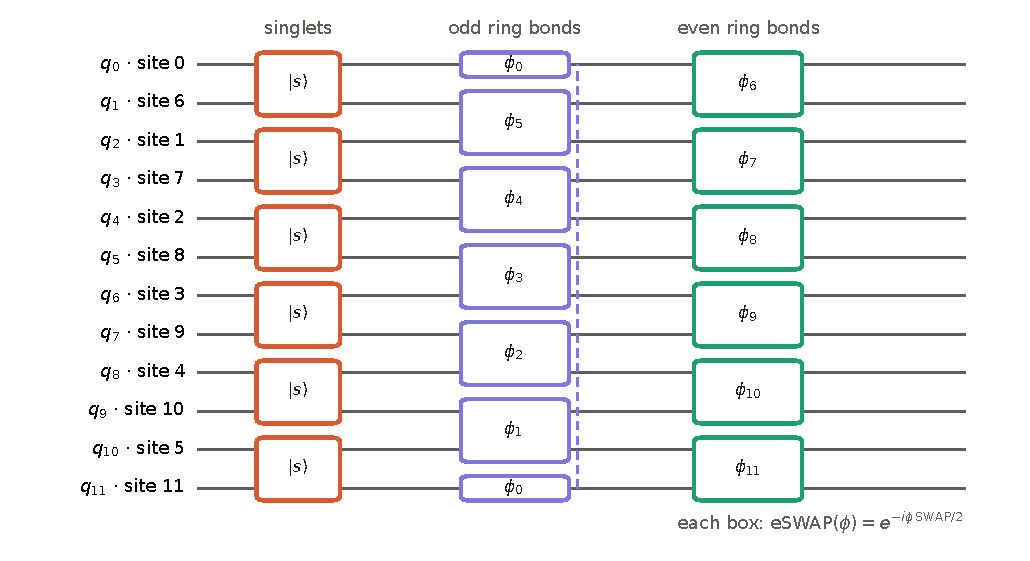
\includegraphics[width=\linewidth]{circuit_rvb}
    \caption{RVB: one angle per bond (12 parameters).}
  \end{subfigure}\\[0.6em]
  \begin{subfigure}{0.72\linewidth}
    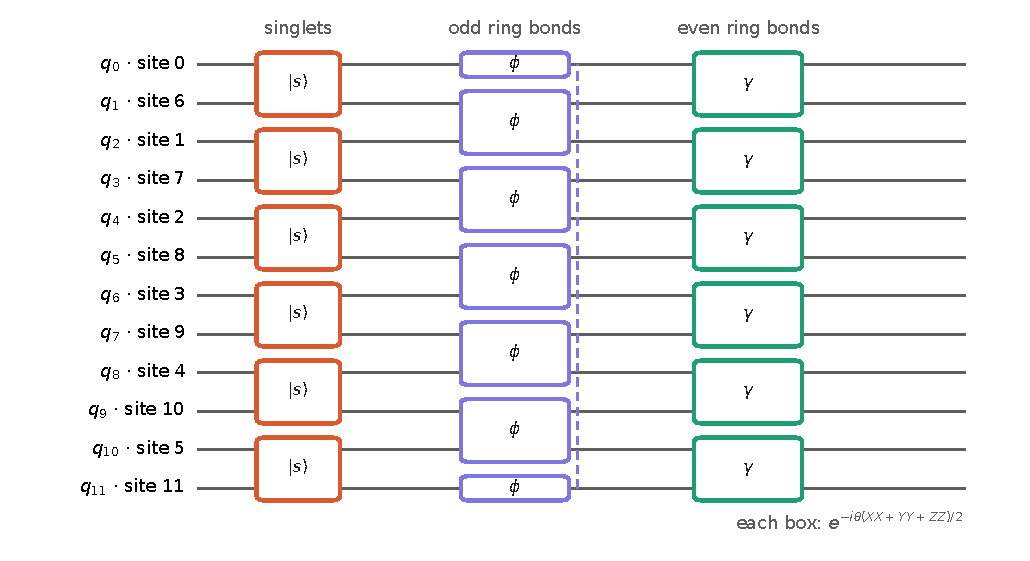
\includegraphics[width=\linewidth]{circuit_hva}
    \caption{HVA: one angle per layer (2 parameters).}
  \end{subfigure}
  \caption{The two ring ansatzes with the default Hamiltonian-cycle site order. Orange: singlet
    preparation on the even ring bonds. Purple: odd-bond layer, including the wrap-around bond
    $(q_{11},q_0)$ drawn as two linked half boxes. Teal: even-bond layer. Every box is the same
    Heisenberg bond evolution; only the parameter sharing differs.}
  \label{fig:circuits}
\end{figure}

\subsection{Why a Hamiltonian cycle}

\begin{thm}*![The ring ansatzes start in the ground space]\label{thm:cycle}
  Let $\sigma$ be the Hamiltonian-cycle order $\sigma=(0,6,1,7,2,8,3,9,4,10,5,11)$. Then
  \begin{enumerate}
    \item the even ring bonds map to the covering $M_1$ and the odd ring bonds to $M_2$;
    \item every ring bond is a lattice bond, and the six hexagon bonds are exactly the lattice
      bonds not on the ring;
    \item $\ket{\psi_{\mathrm{RVB}}(0)}=\ket{\psi_{\mathrm{HVA}}(0,\gamma)}=\ket{D_{M_1}}$ for all
      $\gamma$, with energy $E_0=-18$.
  \end{enumerate}
\end{thm}

\begin{proof}
  (1) $\sigma$ sends $(2k,2k+1)\mapsto\{k,6+k\}\in M_1$ and $(2k-1,2k)\mapsto\{6+k-1,k\}=\{k,6+(k-1)\}\in M_2$,
  including the wrap-around $(11,0)\mapsto\{11,0\}=\{0,6+5\}$. (2) The ring is $M_1\cup M_2$,
  all spokes; the remaining $\VNumBonds-12=6$ bonds are the hexagon. (3) By \cref{lem:eswap}
  $\eSWAP(0)=I$, and $e^{0}=I$, so at $\phi=0$ the state is $\ket{D_\mathcal E}=\ket{D_{M_1}}$ by
  (1). The even layer acts on $\ket{D_{M_1}}$ through bonds $b\in\mathcal E$ that carry its own
  singlets, where $h_b\ket{D_{M_1}}=-3\ket{D_{M_1}}$, so
  $e^{-i\frac\gamma2\Hev}\ket{D_{M_1}}=e^{9i\gamma}\ket{D_{M_1}}$: a global phase. The energy
  is $-18$ by \cref{thm:ground}.
\end{proof}

\begin{prop}[Identity order is hard]\label{prop:identity}
  With $\sigma=\mathrm{id}$, only \VRingFracIdentity{} of the ring bonds and \VSingletIdentity{}
  of the 6 singlet pairs are lattice bonds. Both ansatzes have $E(0)=\VEzeroHvaIdentity$, and the
  global minimum of the HVA energy is $\VHvaMinIdentity$, a relative error of about $40\,\%$
  that no optimiser can remove.
\end{prop}

\begin{proof}
  Identity ring pairs are $\{k,k+1\}$. Lattice bonds among them: the five hexagon bonds
  $\{0,1\},\dots,\{4,5\}$ and $\{11,0\}$, so $6$ of $12$. Of the singlet pairs
  $\{0,1\},\{2,3\},\{4,5\}$ are bonds and $\{6,7\},\{8,9\},\{10,11\}$ are not. At zero
  parameters the state is the singlet product on these pairs: three singlets on bonds give $-9$,
  and every other bond joins two different singlets, contributing $0$ (Exercise in
  \cref{sec:problem}). The minimum is computed in \py{docsgen.physics.hva_minimum} (grid search
  refined by Nelder--Mead on the exact energy); Figure~\ref{fig:landscape} shows the landscape.
\end{proof}

\begin{figure}[H]
  \centering
  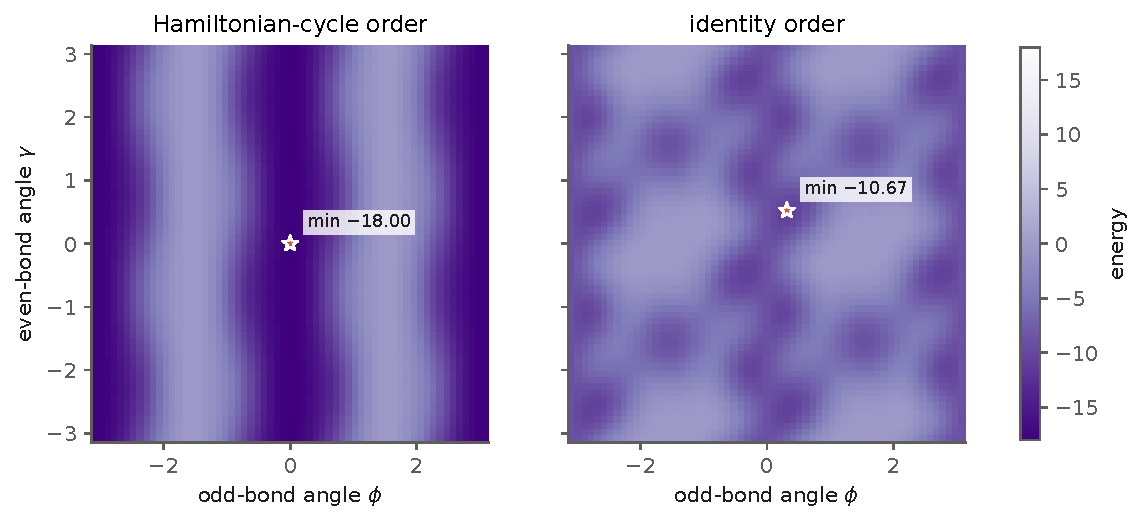
\includegraphics[width=0.86\linewidth]{hva_landscape}
  \caption{Exact HVA energy over $(\phi,\gamma)\in[-\pi,\pi]^2$. Left: Hamiltonian-cycle order.
    The minimum $-18$ is the whole line $\phi=0$ (and $\phi=\pm\pi$, where
    $e^{-i\frac\phi2 h}$ is again trivial up to phase), as \cref{thm:cycle} predicts. Right:
    identity order. The best the ansatz can do is $\VHvaMinIdentity$.}
  \label{fig:landscape}
\end{figure}

Figure~\ref{fig:landscape} is the circuit choice in one picture: the same two-parameter circuit
is exact in one site order and $40\,\%$ off in the other. The minimum on the left is a valley,
not a point, so an optimiser only needs to drive $\phi$ to zero; $\gamma$ is free there.

\begin{rem}[What the 2022 notebook actually did]
  The notebook never transpiled a 12-site Hamiltonian. It hand-wrote a 16-qubit Hamiltonian on
  Guadalupe's physical qubits, whose 12-cycle is the device's heavy-hex loop, and transpiled the
  ring ansatz with an initial layout that is \emph{not} a faithful map of the lattice. Level-3
  routing moved the ring onto the loop anyway, and the V1 \py{Estimator} ignored the circuit
  layout. The result was the Hamiltonian-cycle order by accident. A faithful port with
  \py{observable.apply_layout(layout)} but identity order would silently make the benchmark
  unsolvable (\cref{prop:identity}); this is why \py{site_order} is a first-class, tested
  concept in the package (\py{docs/physics.md}, section~5).
\end{rem}

\begin{rem}[What the circuit does not see]
  Hexagon bonds are never acted on by a gate. That is harmless here, because the ground state
  has no singlets on them, but it makes the ansatz blind to correlations on the hexagon. The
  option \py{ansatz.lattice_aware = true} adds a third HVA sub-layer on those bonds, at the cost of
  routing: kagome contains triangles and heavy-hex does not, so the hexagon bonds can never all be
  physical couplings.
\end{rem}

\subsection*{Exercises}

\begin{exer}
  Show that $e^{-i\frac\phi2 h}$ is trivial up to phase at $\phi=\pi$, and explain the second
  valley at $\phi=\pm\pi$ in Figure~\ref{fig:landscape}.
\end{exer}
\begin{sol}
  $h=2\SWAP-I$, so $e^{-i\frac\pi2h}=e^{i\pi/2}e^{-i\pi\SWAP}$. $\SWAP$ has eigenvalues $\pm1$
  and $e^{\mp i\pi}=-1$, so $e^{-i\pi\SWAP}=-I$. The odd layer is the identity up to phase,
  the state is again $\ket{D_{M_1}}$, and the energy is $-18$ for every $\gamma$.
\end{sol}

\begin{exer}
  How many free parameters does each ansatz have with $\mathrm{reps}=r$ layers, and how many
  bond gates?
\end{exer}
\begin{sol}
  Each layer has 12 bond gates (6 odd, 6 even). RVB: $12r$ parameters; HVA: $2r$ parameters
  ($3r$ with the lattice-aware sub-layer, which adds 6 more gates per layer). Both have $12r$ bond
  gates on the ring.
\end{sol}

\begin{prob}
  Find a site order other than the default for which \cref{thm:cycle} still holds, and
  describe all of them.
\end{prob}
\begin{sol}
  The theorem needs the ring to be a Hamiltonian cycle with the even bonds forming a perfect
  matching. The star has a unique Hamiltonian cycle as an edge set ($M_1\cup M_2$, since a
  Hamiltonian cycle must use both spokes of every degree-2 tip, which is already all 12 spokes).
  Valid orders are its $12$ starting points times $2$ directions. Starting at an odd
  position swaps the roles of $M_1$ and $M_2$, which is equally good by symmetry. So there are 24
  valid site orders, all equivalent.
\end{sol}
